\documentclass[12pt]{article}
\usepackage[margin=1in]{geometry}
\usepackage{graphicx}
\usepackage{courier}
\usepackage{times}
\usepackage[T1]{fontenc}
\usepackage{textcomp}
\usepackage{titlesec}
\newcommand{\sectionbreak}{\clearpage}

\graphicspath{ {img/} }

\begin{document}

\begin{titlepage}
  \begin{center}
    \vspace*{1cm}
    \huge{Integrating IPv6 into the CPE464 Lab Curriculum}

    \vspace{1.5cm}

    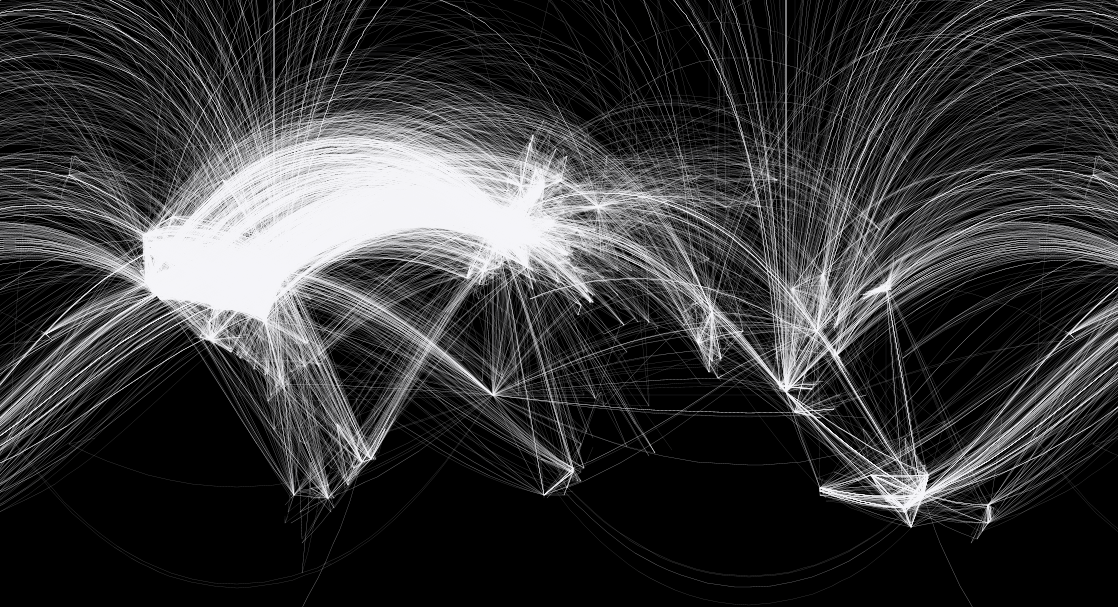
\includegraphics[width=1\textwidth]{internet_map.png}
    \vfill
    \large{
      Jacob Hladky\\
      California Polytechnic State University\\
      San Luis Obispo, CA\\
      \texttt{jhladky@calpoly.edu}
    }

    \vspace{1cm}

    \today   
  \end{center}
\end{titlepage}

\pagenumbering{roman}

\tableofcontents

\listoffigures
\listoftables

\pagenumbering{arabic}

\section{Introduction}
The Internet Protocol, version 4, was standardized in 1981 by DARPA, a division of the Department of Defense focused on developing cutting-edge technologies. The protocol, designed to connect every computer on the globe, had an ``address-space'' of roughly 4 billion hosts, a number which seemed unbelievely immense compared to the 200 or so computers on the internet at the time.\\\\
On 4th of July of this year the American Registry for Internet Numbers is predicted to exhaust its remaining IPv4 addresses. Registries in Asia (APNIC), and Europe (RIPE NCC) have already run out of their share of the address space. A replacement protocol, IPv6 was designed and approved in 1998. Adoption has been slow, but is rapidly increasing as more and more countries run out of addresses.\\\\
Cal Poly students taking CPE464, Introduction to Computer Networks, will learn IPv4 in depth. They will learn static routing, RIP, DHCP, and countless other critical components of the internet. But they will not learn about IPv6. As more and more businesses adapt IPv6, familiarity with the new Internet Protocol is becoming more and more crucial.\\\\
This report will present research about the best way to integrate the teaching of IPv6 into the CPE464 lab curriculum. This question can be split into two parts: the first, of which technology implementing IPv6 best shows the features of the new protocol, and the second, of what method of presenting this technology will be the most effective. This report will answer both questions in the form of recommending a new IPv6 lab curriculum.\\\\
The methods section will discuss how data was obtained for the report, and the results will present the findings of that data. The conclusions and recommendations sections detail the new curriculum and the recommendations that can be derived from it. Finally, a glossary of terms provides definitions for any unfamiliar terms used here, and the works cited provides links to the research done on IPv6.

\section{Methods}
aaaa

\section{Results}
aaaa

\section{Conclusions}
aaaa

\section{Recommendations}
aaaa

\section{Glossary of Terms}
aaaa

\section{Works Cited}
aaaa

\end{document}



